\documentclass[12pt]{article}

% Variables
\newcommand{\thedate}{March 1, 2012}
\newcommand{\assignment}{CS280 - Spring 2012 HW2}

% Formatting packages
\usepackage{palatino}
\usepackage{fullpage}
\usepackage{fancyhdr}
\usepackage{enumerate}
\usepackage{algorithmic}
\usepackage{pgf}
\usepackage{tikz,tkz-euclide}
\usetkzobj{all}
\usepackage{qtree}
\usetikzlibrary{arrows,automata}

% Math tools
\usepackage{mathtools}
\usepackage{amssymb}
\usepackage{gensymb}
\usepackage{xfrac}

% CS tools
\usepackage{algorithmic}
\usepackage[options]{mcode}

% Header Settings
\pagestyle{fancy}
\headsep = 35pt
\setlength{\headheight}{20pt}


% Header
\rhead{\textsc{Eric Tzeng, Brandon Wang \\\footnotesize{\thedate} \\}}
\lhead{\Large \textsc{\assignment}}
\cfoot{\large\thepage}

% Numbered environments
\newtheorem{theorem}{Theorem}[section]
\newtheorem{lemma}[theorem]{Lemma}
\newtheorem{proposition}[theorem]{Proposition}
\newtheorem{corollary}[theorem]{Corollary}

% Unnumbered environments
\newenvironment{proof}[1][Proof]{\begin{trivlist}
\item[\hskip \labelsep {\bfseries #1}]}{\end{trivlist}}
\newenvironment{definition}[1][Definition]{\begin{trivlist}
\item[\hskip \labelsep {\bfseries #1}]}{\end{trivlist}}
\newenvironment{example}[1][Example]{\begin{trivlist}
\item[\hskip \labelsep {\bfseries #1}]}{\end{trivlist}}
\newenvironment{remark}[1][Remark]{\begin{trivlist}
\item[\hskip \labelsep {\bfseries #1}]}{\end{trivlist}}

% QED Symbol
\newcommand{\qed}{\nobreak \ifvmode \relax \else
      \ifdim\lastskip<1.5em \hskip-\lastskip
      \hskip1.5em plus0em minus0.5em \fi \nobreak
      \vrule height0.75em width0.5em depth0.25em\fi}

% Start of document
\begin{document}
\section*{Q1}
  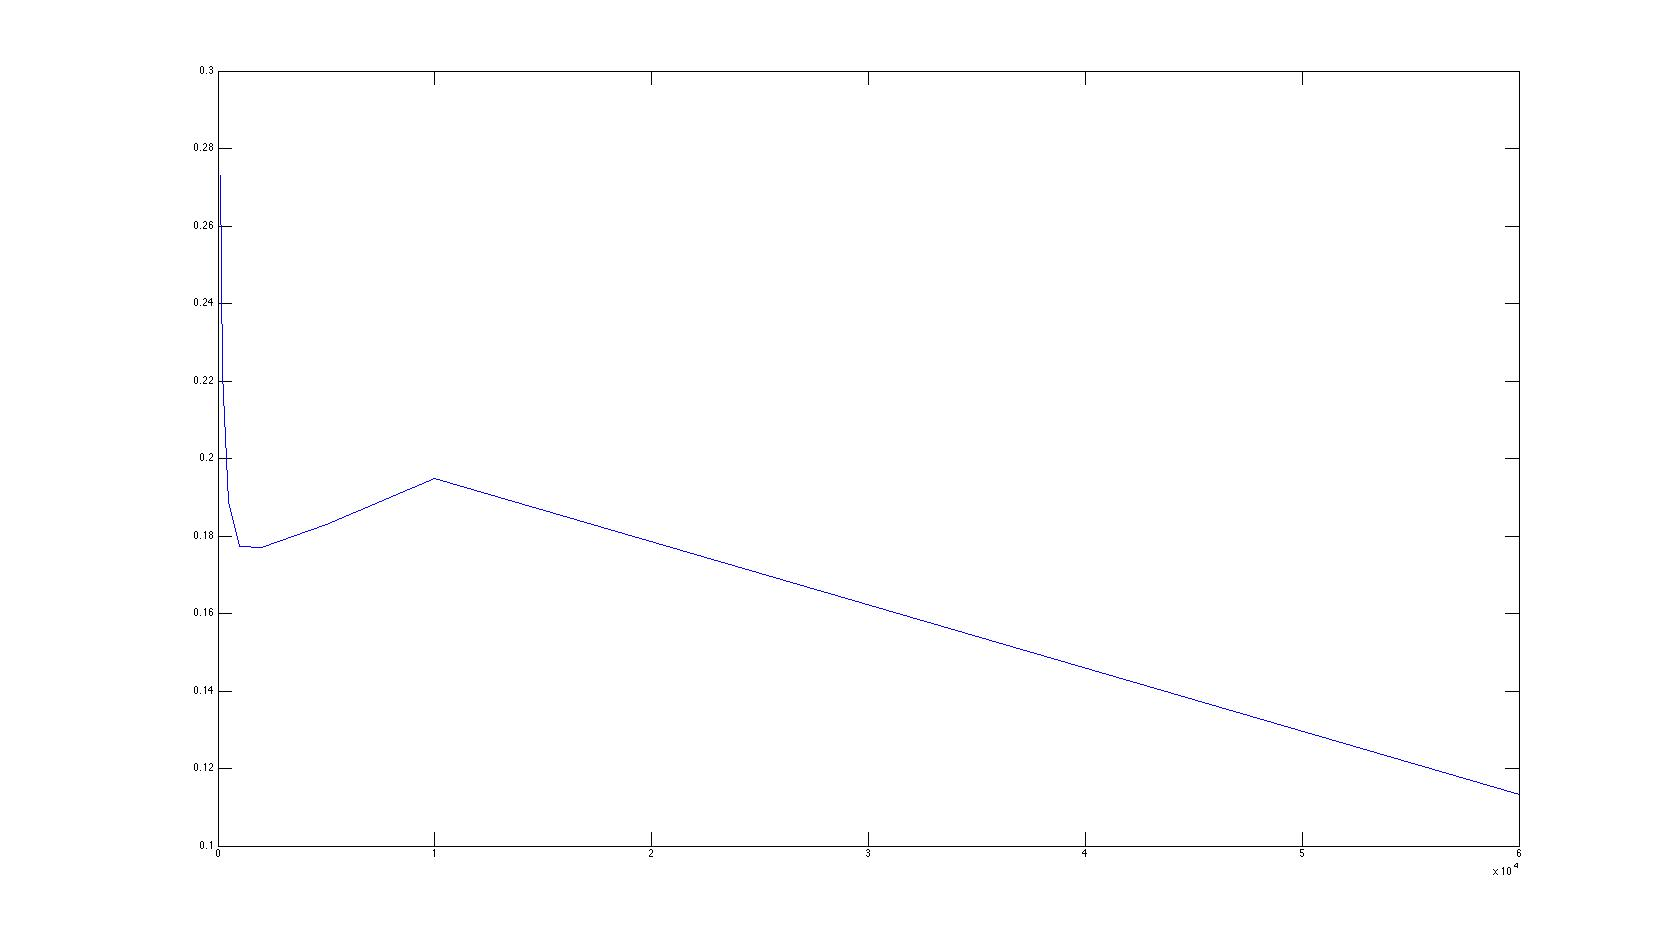
\includegraphics[scale=0.3]{q1_pixel_error.jpg}
  \begin{tabular}{l|l}
    \hline
    Training Samples & Error Rate \\
    \hline
    100   & 0.2731 \\
    200   & 0.2219 \\
    500   & 0.1889 \\
    1000  & 0.1774 \\
    2000  & 0.177  \\
    5000  & 0.1829 \\
    10000 & 0.1949 \\
    60000 & 0.1134 \\
  \end{tabular}
\section*{Q2}
  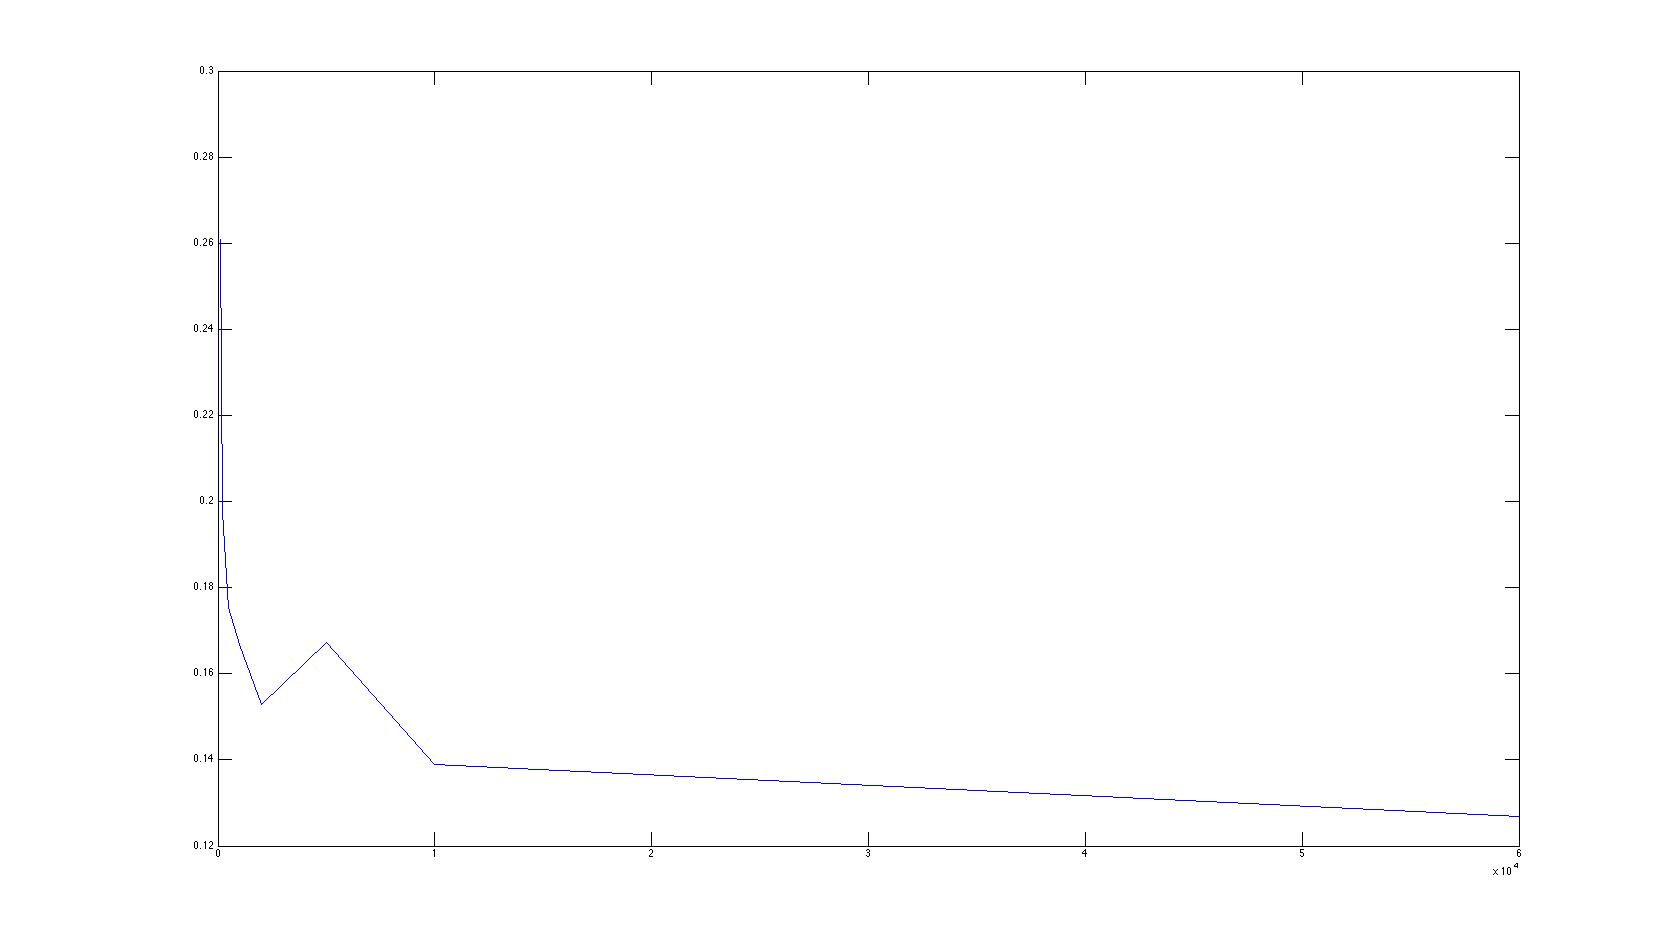
\includegraphics[scale=0.3]{q2_full.jpg}
  \begin{tabular}{l|l}
    \hline
    Training Samples & Error Rate \\
    \hline
    100   & 0.2608 \\
    200   & 0.1975 \\
    500   & 0.1754 \\
    1000  & 0.1667 \\
    2000  & 0.1528 \\
    5000  & 0.1672 \\
    10000 & 0.139 \\
    60000 & 0.1269 \\
  \end{tabular}

\end{document}
